\subsection{垃圾分类}

法国的垃圾需要严格分类才可以丢弃,随意丢弃垃圾可能会收到罚款。常见的垃圾分为:

\begin{itemize}
    \item 可回收垃圾(Déchets recyclables):包装盒、塑料袋、塑料瓶、金属等散装放入黄色的垃圾桶。玻璃瓶放入玻璃制品特定的垃圾桶。
    \item 普通垃圾:无法回收的家庭垃圾,放入密封垃圾袋丢到灰色或棕色垃圾桶。
    \item 可降解垃圾:如厨余、果皮、蔬菜残渣、茶叶渣等,可以投入指定的可降解垃圾桶,进而进行堆肥处理。请主要注意不要将塑料袋等不可降解物品放入可降解垃圾桶。
    \item 旧衣物及纺织品:请投放至专门的旧衣物回收箱(通常分布在小区、超市或市政指定地点),用于再利用或环保处理。
    \item 有害垃圾:包括药品、电池、电器、灯管等有害垃圾需要丢弃到专门的回收地点,请查看居住城市的相关规定。
    \item 废旧家具:请查看居住城市的相关规定,一般情况下每个月或每个礼拜会有固定的时间统一回收。
    \item 装修垃圾:需要自行送到垃圾处理厂,请查看居住城市的相关规定。
\end{itemize}

\begin{figure}[h]
    \centering
    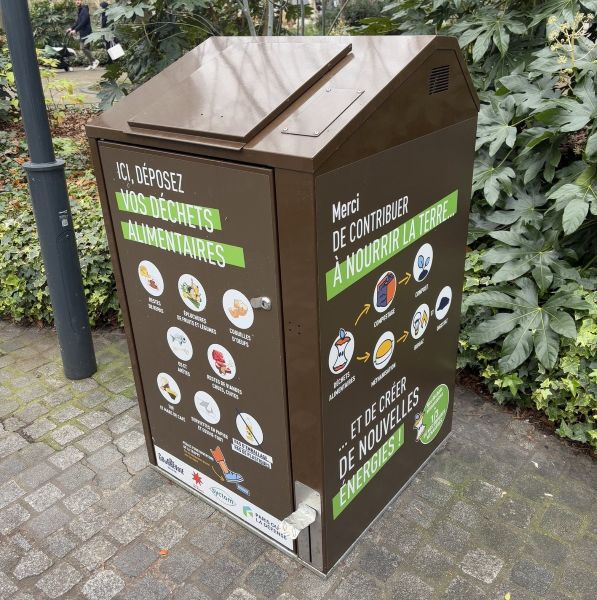
\includegraphics[width=0.4\textwidth]{chapters/06_life/images/garbage_bin_biodegradable.jpg}
    \caption{法国常见的可降解垃圾桶示例}
\end{figure}

\begin{figure}[h]
    \centering
    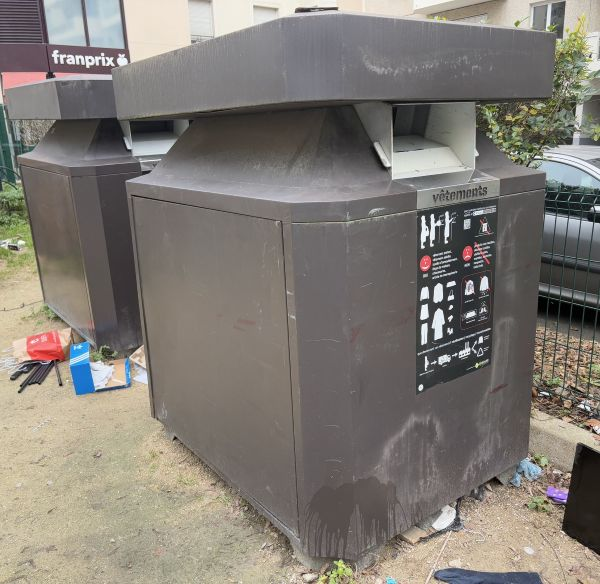
\includegraphics[width=0.4\textwidth]{chapters/06_life/images/garbage_bin_clothes.jpg}
    \caption{法国常见的旧衣物回收箱示例}
\end{figure}

\textbf{温馨提示:}请遵守当地垃圾分类规定,正确投放垃圾,避免因分类错误而被罚款。部分城市对垃圾投放时间和垃圾袋有特殊要求,请提前了解相关信息。

